%\documentclass[colorBG,slideColor,fyma]{beamer}
\documentclass[xcolor=dvipsnames]{beamer}
\setbeamertemplate{navigation symbols}{}
\usepackage{amsmath}
\usepackage{amsfonts}
\usepackage{latexsym}
\usepackage{amssymb}
\usepackage{xypic}
\usepackage{epsfig}
\usepackage{subcaption}
\usepackage{xcolor}
\graphicspath{ {./img/} }

\usecolortheme[named=Brown]{structure}
\usetheme{Boadilla}

\def\xcolorversion{2.00}
\def\xkeyvalversion{1.8}
\usepackage[version=0.96]{pgf}
\usepackage{tikz}
\usetikzlibrary{arrows,shapes,snakes,automata,backgrounds,petri}

\title[]{Person Identification using Gait Analysis}
 \author{Siddharth S\\Rahul Rajagopalan\\  \hspace{0.1cm}\\Supervisor: Dr.Sakaya Milton R}
\institute[SSNCE]{Department of Computer Science and    Engineering\\ SSN College of Engineering, Chennai
}
\date{February 10, 2024}

% Some new environments for the paper
%
\newtheorem{dfn}{Definition}[section]
\newtheorem{prop}[dfn]{Proposition}
\newtheorem{lem}[dfn]{Lemma}
\newtheorem{thm}[dfn]{Theorem}
\newtheorem{cor}[dfn]{Corollary}
\newtheorem{clm}[dfn]{Claim}
%\newtheorem{fact}[dfn]{Fact}
\newtheorem{ex}[dfn]{Exercise}
\newtheorem{eg}[dfn]{Example}
%
%\newcommand{\RightBox}{\begin{flushright} $\Box$ \end{flushright}}
\newcommand{\RightBox}{{\phantom{a}}\hfill $\Box$ \\}
%\newenvironment{proof}{{\bf Proof:~}}{\RightBox}
\newenvironment{prf}{{\bf Proof~Idea:~}}{\RightBox}
%\newcommand{\claim}[1]{{\bf Claim #1:~}}
%
\newcommand{\Dfn}[1]{Definition \ref{dfn:#1}}
\newcommand{\Prop}[1]{Proposition \ref{prop:#1}}
\newcommand{\Lem}[1]{Lemma \ref{lem:#1}}
\newcommand{\Thm}[1]{Theorem \ref{thm:#1}}
\newcommand{\Cor}[1]{Corollary \ref{cor:#1}}

%Action-indexed diamond modality
\newcommand{\Adiam}[1]{\mbox{$\langle #1 \rangle$}}
\newcommand{\diamin}{\Diamond\kern-0.5em{\raisebox{.25ex}{\rm -}}\kern0.175em}
\newcommand{\until}{\mbox{\large\bf U}}
\newcommand{\since}{\mbox{\large\bf S}}
\newcommand{\nxt}{\mbox{$\bigcirc$}}
\newcommand{\nxtdot}{\displaystyle \bigodot}
\newcommand{\past}{\diamin}
\newcommand{\ifpast}{\mbox{$\boxminus$}}
\newcommand{\now}{\mbox{$\langle now \rangle$}}
\newcommand{\Now}{\mbox{$[now]$}}
\newcommand{\pres}{\mbox{$\rangle \langle$}}
\newcommand{\snd}{\mbox{\large\bf s}}
\newcommand{\rec}{\mbox{\large\bf r}}
\newcommand{\nc}{\mathbf{no\_comm}}

%Propositional connectives
%\newcommand{\implies}{{\raisebox{.20ex}{$\scriptstyle ~\supset~$}}}
\newcommand{\Imply}{~~\mathbf{\supset}~~}
\newcommand{\Not}{\mbox{$\lnot$}}
\newcommand{\xor}{\mathbf{\oplus}}
\newcommand{\True}{\mathit{True}}
\newcommand{\False}{\mathit{False}}

%Large symbols
\newcommand{\andover}{\displaystyle \bigwedge}
\newcommand{\orover}{\displaystyle \bigvee}
\newcommand{\capover}{\displaystyle \bigcap}
\newcommand{\cupover}{\displaystyle \bigcup}
\newcommand{\piover}{\displaystyle \Pi}
\newcommand{\ohat}[1]{\widehat{#1}}
\newcommand{\otilde}[1]{\widetilde{#1}}
\newcommand{\obar}[1]{\overline{#1}}
\newcommand{\Sigtil}{\mbox{$\otilde{\Sigma}$}}
\newcommand{\DA}{\mbox{$\Sigtil~=~(\Sigma_1, \dots, \Sigma_n)$}}

%Useful symbols
\newcommand{\derives}{\vdash}
\newcommand{\defn}{\mbox{$~\stackrel{\rm def}{=}~$}}
\newcommand{\qneq}{\mbox{$~\stackrel{\rm ?}{=}~$}}
\newcommand{\eqv}{\approx}
\newcommand{\hash}{\sharp}
\newcommand{\restr}{\lceil}
%\newcommand{\bot}{\bottom}
\newcommand{\nat}{{\bf N}}
\newcommand{\pfin}[1]{\mbox{$\wp_{fin}(#1)$}}
%\newcommand{\mod}[1]{\mbox{$|#1|$}}
\newcommand{\memb}[2]{\mbox{${#1} \in {#2}$}}
\newcommand{\E}{\mathbf{E}}



%Some roman words in math mode
\newcommand{\Iff}{\Leftrightarrow}
\newcommand{\For}{\mbox{~for~}}
\newcommand{\Where}{\mbox{~where~}}
%\newcommand{\And}{\mbox{~and~}}
\newcommand{\Implies}{\Rightarrow}

%Relations

% structures
\newcommand{\Sigstr}{\mbox{$\Sigma^*$}}
\newcommand{\TS}{\mbox{$TS = (Q,\to)$}}  %generates TS=(Q,->)
\newcommand{\TSP}{\mbox{$TS = (Q,\To)$}}         %generates TS=(Q,=>)
\newcommand{\TSi}{\mbox{$TS_i = (Q_i,\to_i)$}}           
\newcommand{\TSE}{\mbox{$TS_{ES}$}}
\newcommand{\TSN}{\mbox{$TS_{\cal N}$}}
\newcommand{\ES}{\mbox{$ES = (E,\leq,\#)$}}       %generates ES=(E,<=,#)
\newcommand{\LES}{\mbox{$ES = (E,\leq,\#,\phi)$}} %generates ES=(E,<=,#,phi)
\newcommand{\Tmdl}{\mbox{$M = (TS,V)$}}          %generates M = (TS,V)
\newcommand{\cfin}[1]{\mbox{$C_{#1}$}}           %finite configurations of
\newcommand{\fincon}[1]{\mbox{$C_{#1}^{fin}$}}  %finite configurations

% classes
\newcommand{\mdl}[1]{\mbox{${\cal M}_{#1}$}}%generates script M with subscript
\newcommand{\dmodels}{\mbox{$\models_{Det}~$}}

% For transitions steps
\newcommand{\step}[1]{\mbox{$\stackrel{#1}{\to}$}}
\newcommand{\Funnyto}{\rightsquigarrow}
\newcommand{\longstep}[1]{\mbox{$\stackrel{#1}{\longrightarrow}$}}
\newcommand{\emptystep}{\step{\emptyset}}
\newcommand{\reach}[1]{\mbox{${\cal R}(#1)$}}
\newcommand{\reachin}[2]{\mbox{${\cal R}_{#1}(#2)$}}

% For a "double-lined" transition relation
\newcommand{\To}{\Rightarrow}
\newcommand{\From}{\Leftarrow}
\newcommand{\Step}[1]{\mbox{$\stackrel{#1}{\To}$}}
\newcommand{\Longstep}[1]{\mbox{$\stackrel{#1}{\Longrightarrow}$}}
\newcommand{\Longlongstep}[1]{\mbox{$\stackrel{#1}{\Longlongrightarrow}$}}
\newcommand{\Emptystep}{\Step{\emptyset}}

% Net theory
\newcommand{\presca}[1]{\mbox{${ }^{\bullet}#1$}}
\newcommand{\postsca}[1]{\mbox{$#1 \, { }^{\bullet}$}}%

%The built in downarrow generates too much space after it
%\newcommand{\down}{\mbox{$\downarrow \!$}}
\newcommand{\down}{\mbox{$\downarrow$}}
\newcommand{\up}{\mbox{$\uparrow \!$}}
\newcommand{\ldot}{{\rm <}\kern-0.37em{\raisebox{.25ex}{\bf .}}\kern0.375em}

%Trace theory
\newcommand{\edoti}{\mbox{$\doteq_I$}}
\newcommand{\eqi}{\mbox{$=_I$}}
\newcommand{\edotk}{\mbox{$\doteq_k$}}
\newcommand{\eqk}{\mbox{$=_k$}}

\newcommand{\calL}{\mathcal{L}}
\newcommand{\calB}{\mathcal{B}}
\newcommand{\posetlang}[1]{\mbox{${\calL}^{po}(#1)$}}%poset language of an SCA
\newcommand{\bddlang}[2]{\mbox{${{\calL}^{#1}}(#2)$}} %bounded buffer language

\newcommand{\calS}{\mathcal{S}}
\newcommand{\calA}{\mathcal{A}}
\newcommand{\calC}{\mathcal{C}}
\newcommand{\calE}{\mathcal{E}}
\newcommand{\calG}{\mathcal{G}}



\newcommand{\calQ}{\mathcal{Q}}
\newcommand{\calD}{\mathcal{D}}
\newcommand{\calCN}{\mathcal{CN}}
\newcommand{\calI}{\mathcal{I}}
\newcommand{\calF}{\mathcal{F}}
\newcommand{\calM}{\mathcal{M}}

\begin{document}
\begin{frame}
\maketitle
\end{frame}


\AtBeginSection[]{
\begin{frame}{beamer}
\frametitle{Outline}
\tableofcontents[currentsection]
\end{frame}
}

\begin{frame}{Introduction}
\begin{itemize}
\item Gait refers to an individual's walking style based on the motion of their limbs.
\item Gait analysis is the study of human walking patterns which can be used in fields such as security, forensics, etc.
\item It can be used as a biometric, as each individual's gait is unique from one another.
\end{itemize}
\end{frame}

\begin{frame}{Motivation}
\begin{itemize}
\item Person identification using gait analysis is a promising tool that enhances security.
\item  It doesn't require physical contact or the person's cooperation, making it a valuable tool for surveillance and security applications.
\item It can significantly aid law enforcement agencies in identifying
and tracking suspects
\end{itemize}
\end{frame}

\begin{frame}{Problem Statement}
\begin{itemize}
\item To identify people using {\bf gait analysis} in an {\bf uncooperated environment}, even in cases involving {\bf covariate factors} such as {\bf baggage} and {\bf clothing conditions}.
\item Using {\bf Gait Energy Images (GEIs)} as input.
 

\end{itemize}
\end{frame}

\begin{frame}{Literature Survey}
\begin{table}
  \centering
  
  \tiny
  \begin{tabular}{|p{3cm}|p{5cm}|p{3cm}|} 
    \hline
    Paper & Methodology & Limitations \\
    \hline
    A smart surveillance system for uncooperative gait recognition using cycle-consistent generative adversarial networks\cite{alsaggaf2021}.
    & 
    Uses cycle-consistent GANS to eliminate covariate factors .
    Makes use of cycle consistency loss.
    Uses CNN for person identification.
    Accuracy - 79\% in carrying conditions and 52\% in clothing conditions & 
    Inadequate accuracy in clothing conditions
    \\

    \hline
  \end{tabular}


   \begin{tabular}{|p{3cm}|p{5cm}|p{3cm}|}
    Learning to discover
    cross-domain relations with generative adversarial networks \cite{kim2017}. &
    Reconstruction loss is used instead of the normal cycle loss. 
    Two reconstruction losses ($Lrecon_{a}$ and $Lrecon_{b}$) are calculated separately and used to fine-tune their respective generators. &
    Susceptible to mode collapse, complex training and hyperparameter tuning.\\
    \hline
  \end{tabular}


   \begin{tabular}{|p{3cm}|p{5cm}|p{3cm}|}
    Wasserstein generative adversarial networks \cite{arjovsky2017}.&
    Uses Wasserstein distance as a new loss function instead of traditional GAN loss.
    Measures the difference between the distributions of true and fake images. &
    Complex to implement compared to traditional GANs and
    sensitive to hyperparameter tuning.\\
    \hline
  \end{tabular}


  \begin{tabular}{|p{3cm}|p{5cm}|p{3cm}|}
    Deep learning-based gait recognition using smartphones in the wild\cite{zou2020}.&
    Used integrated sensors such as accelerometers and gyroscopes. Uses the whuGAIT dataset. DCNN and LSTM are used to learn the spatial and temporal features, and perform information fusion giving an accuracy of 90.22\% for classifying walking and non-walking data.&
    The proposed methods are based on the dataset containing 118 healthy people. Therefore, it does not give proper results on people with physical problems.\\
    \hline
    
  \end{tabular}

  \begin{tabular}{|p{3cm}|p{5cm}|p{3cm}|}
    Human gait recognition subject to different covariate factors in a multi-view environment\cite{asif2022}.&
    Human gait recognition is subject to different covariate factors in a multi-view environment. A set of gait images representing normal walking, walking with changed clothes, and walking with carrying bags used as input. A validated SVM model is applied . Uses CASIA-B dataset. The overall accuracy achieved through the proposed method is 83.33\%.&
    The accuracy of a normal walk is lesser compared to walking with different clothes.\\
    \hline
  \end{tabular}
  
\end{table}
\end{frame}

\begin{frame}{Literature Survey}
\begin{table}
  \centering
  
  \tiny
  \begin{tabular}{|p{3cm}|p{5cm}|p{3cm}|} 
    \hline
    Paper & Methodology & Limitations \\
    \hline
    Gait image classification using Deep Learning Models for medical diagnosis\cite{vasudevan2023}.
    & 
    Gait Image Classification Using Deep Learning Models for Medical Diagnosis and comparing effectiveness of various models. Silhouette image data is taken as input. Uses CNN-LSTM model for classifying the gait silhouette images. Transfer learning models such as MobileNetV2, InceptionV3,etc are used. Uses CASIA-B and CASIA-C. CNN-LSTM - accuracy of 87.25\%.& 
    Model complexity is high and time consuming. High computational set up required.
    \\

    \hline
  \end{tabular}


   \begin{tabular}{|p{3cm}|p{5cm}|p{3cm}|}
    Human gait recognition for biometric application using Bayesian optimization and extreme learning machine  \cite{khan2023}. &
    Motion regions are initially extracted using optical flow, followed by training two models based on EfficientNet-B0 architecture: one using these motion regions and another using enhanced video frames. Bayesian Optimization dynamically selects hyperparameters during training. Sq-Parallel Fusion (SqPF) combines features from both models, while the Tiger optimization algorithm is enhanced as Entropy Variance controlled Tiger optimization (EVcTO). Finally, an extreme learning machine (ELM) classifier is employed to classify the best-selected features. Uses Casia B dataset. &
    Did not perform well for 54 and 108 degrees due to high intra-class similarity.
.\\
    \hline
  \end{tabular}


   \begin{tabular}{|p{3cm}|p{5cm}|p{3cm}|}
    Real-time human recognition at night via integrated face and gait recognition technologies\cite{manssor2021}.&
    It uses a combination of facial and gait recognition to identify people, especially at night. The two features are processed separately using the YOLOv3 model and combined. The Thermal Infrared (TIR) image is optimized using the OTI-Net. The features are extracted using PDM-Net. Finally, the PRM-Net is used to recognize humans. Uses DHU Night dataset. Accuracy - 90\% gait detection.
  &
    The accuracy is decreased if the face is covered and the body is concealed by clothing. A high computational setup is needed. Carrying conditions not taken into consideration.\\   
    \hline
  \end{tabular}

 
  
\end{table}
\end{frame}



\begin{frame}{Literature Survey}

\begin{table}
  \centering
  
  \tiny % Set the font size to small

  \begin{tabular}{|p{3cm}|p{5cm}|p{3cm}|}
  \hline
    Paper & Methodology & Limitations \\
    \hline
    Learning 3D spatiotemporal gait feature by convolutional network for person identification.\cite{huynh2020}.&
    A model-based approach where feature extraction is done using various joint distances and joint angles to capture dynamics of human pose in the spatial and temporal domains. DCNN is used for person identification. Accuracy -  87.63\%. Uses  KS20 VisLab Multi-View Kinect Skeleton Dataset. &
    Does not work well with dynamic environments and with covariate factors.\\
    \hline
    
  \end{tabular}
  
   \begin{tabular}{|p{3cm}|p{5cm}|p{3cm}|}
    Multi-view gait Recognition Based on Generative Adversarial Network to achieve robust gait recognition by extracting invariant features and retaining identity information during view transformation. \cite{wen2022}.&
    GAN was used to convert the gait image of any states and views to the normal state of 54°, 90°, 126° as GEI is clear in those angles. A multi-view gait recognition model was constructed based on the deep convolutional network. Uses the Casia B dataset and outputs an accuracy- 77.84\% for bag and 50.37\% for coat sequence.&
    The accuracy is not sufficient due to the limitations of employing a basic GAN architecture.\\
    \hline
  \end{tabular}

  \begin{tabular}{|p{3cm}|p{5cm}|p{3cm}|}
    A model-based gait recognition method with body pose and human prior knowledge \cite{liao2020}.&
    Human pose is converted from 2D to 3D to perform feature extraction of the spatial and temporal features. 4 main features - limb, angle, pose, and motion are extracted and sent through a CNN for identification. Uses a model-based approach.&
    High computational setup. Not suitable for dynamic environments.  \\
    \hline
  \end{tabular}

  \begin{tabular}{|p{3cm}|p{5cm}|p{3cm}|}
    Unpaired image-to-image translation using cycle-consistent adversarial networks \cite{zhu2017}.&
    CycleGAN is used to translate an image of a zebra to a horse and vice versa. The loss functions taken into consideration are the adversarial loss and cycle consistency loss.&
    Has not been used in GAIT-relevant applications.  \\
    \hline
  \end{tabular}

\end{table}
    
    
\end{frame}

\begin{frame}{Justification for the problem formulation}

\begin{itemize}
\item Previous studies in gait analysis for person identification have achieved good accuracy under carrying conditions but struggled to deliver satisfactory results in {\bf clothing conditions (52\%}).
\item The use of unsupervised image-to-image translation GANs in this context is limited.
\item  Aim to address the challenges associated with clothing conditions and enhance the overall performance of
gait analysis for person identification.

\end{itemize}
\end{frame}

\begin{frame}{Feasibility Study}
    \begin{itemize}
        \item Have access to an existing dataset, {\bf CASIA-B - 124 subjects}; {\bf 6 normal} walk conditions, {\bf 2 carrying} conditions, and {\bf 2 clothing} conditions for each subject; each condition having over 50 images in {\bf 10 different angles}. It has a total of {\bf 19139} images.
        \item The project’s scalability is a key strength, as it can be potentially extended to real-time surveillance applications.
        \item  With the existing dataset and by utilizing existing platforms like Colab or Kaggle, we ensure that the implementation of the project is feasible. 
    \end{itemize}
\end{frame}

\begin{frame}{GEI Images}

\begin{figure}[!h]
    \centering
    \begin{subfigure}{0.3\textwidth}
        \centering
        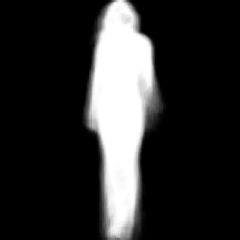
\includegraphics[width=0.4\textwidth]{walk-nm1.jpg}
        
        \label{fig:img1}
    \end{subfigure}
    \begin{subfigure}{0.3\textwidth}
        \centering
        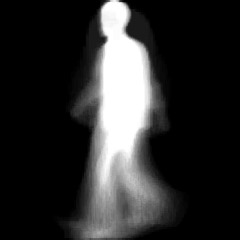
\includegraphics[width=0.4\textwidth]{walk-nm2.jpg}
        
        \label{fig:img2}
    \end{subfigure}
    \caption{GEI involving normal walk}
    
\end{figure}

\begin{figure}[!h]
    \centering
    \begin{subfigure}{0.3\textwidth}
        \centering
        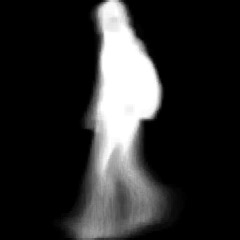
\includegraphics[width=0.4\textwidth]{walk-bg1.jpg}
        
        \label{fig:img1}
    \end{subfigure}
    \begin{subfigure}{0.3\textwidth}
        \centering
        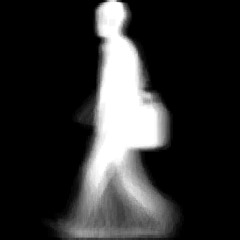
\includegraphics[width=0.4\textwidth]{walk-bg2.jpg}
        
        \label{fig:img2}
    \end{subfigure}
    \caption{GEI involving bags}
  \end{figure}


  \begin{figure}[!h]
    \centering
    \begin{subfigure}{0.3\textwidth}
        \centering
        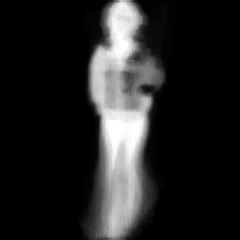
\includegraphics[width=0.4\textwidth]{walk-cl1.jpg}
        
        \label{fig:img1}
    \end{subfigure}
    \begin{subfigure}{0.3\textwidth}
        \centering
        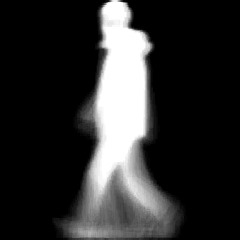
\includegraphics[width=0.4\textwidth]{walk-cl2.jpg}
        
        \label{fig:img2}
    \end{subfigure}
    \caption{GEI involving clothes}
  \end{figure}
    
\end{frame}

\begin{frame}{Existing System}
    \begin{figure}
    \centering
    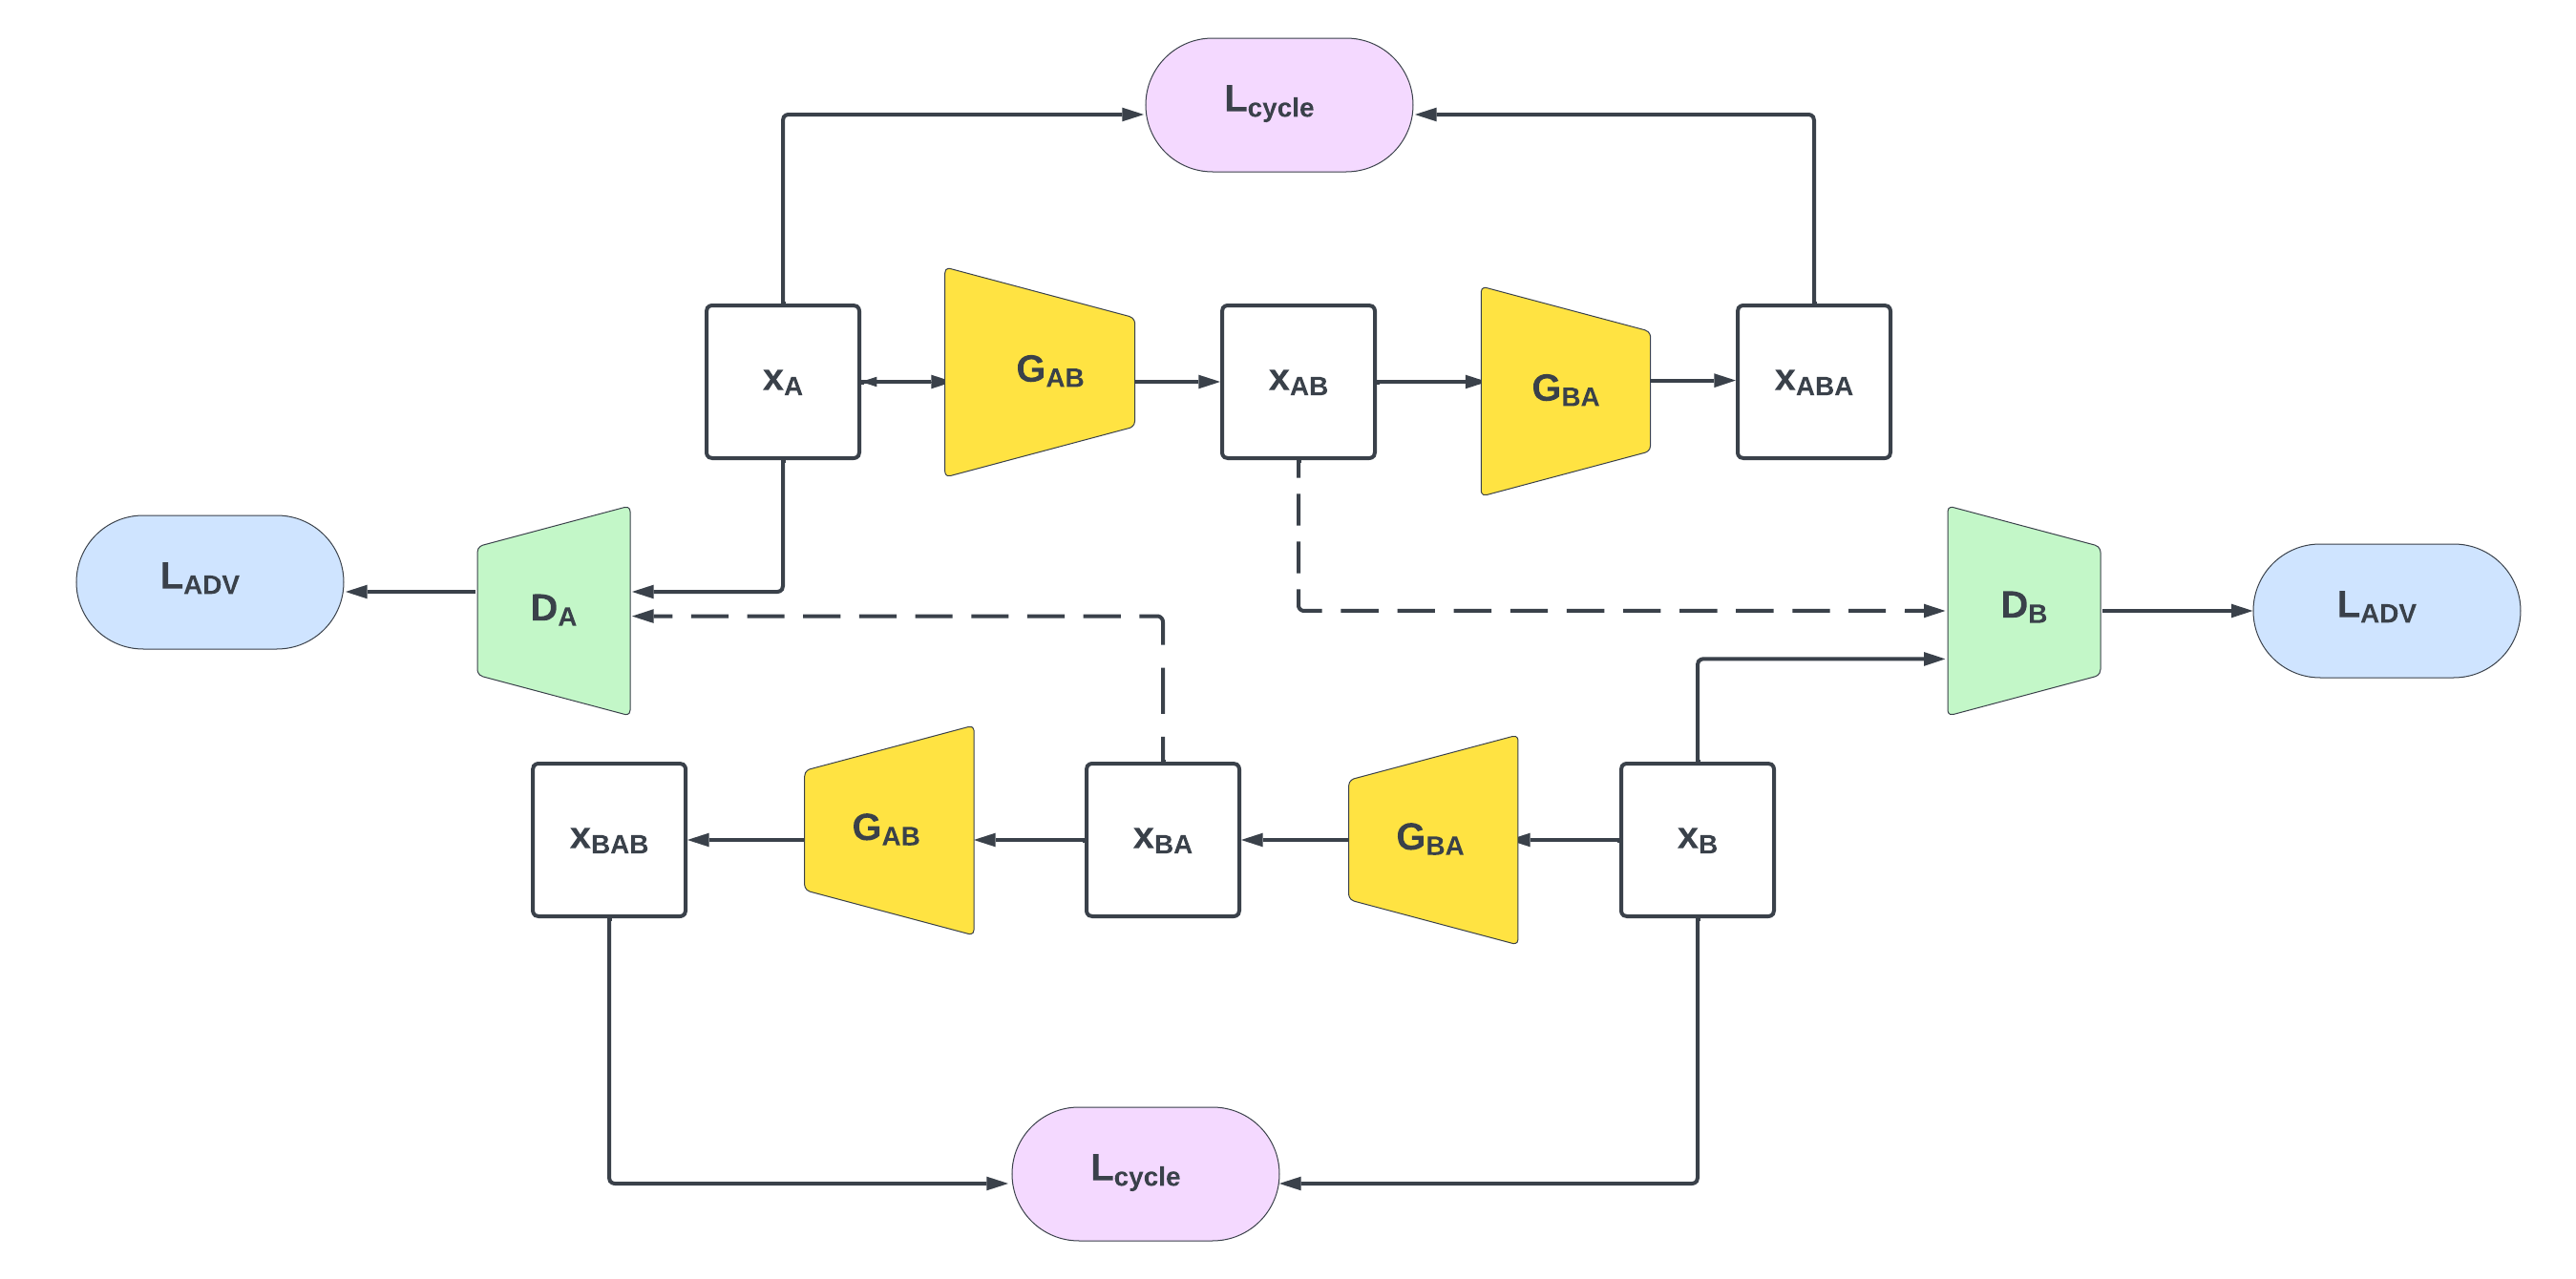
\includegraphics[scale = 0.28]{ppt/img/color-cc.png}
    \caption{Architecture of cycle consistent GAN}
    \label{fig:enter-label}
\end{figure}
\end{frame}

\begin{frame}{Proposed System}
\begin{figure}
    \centering
    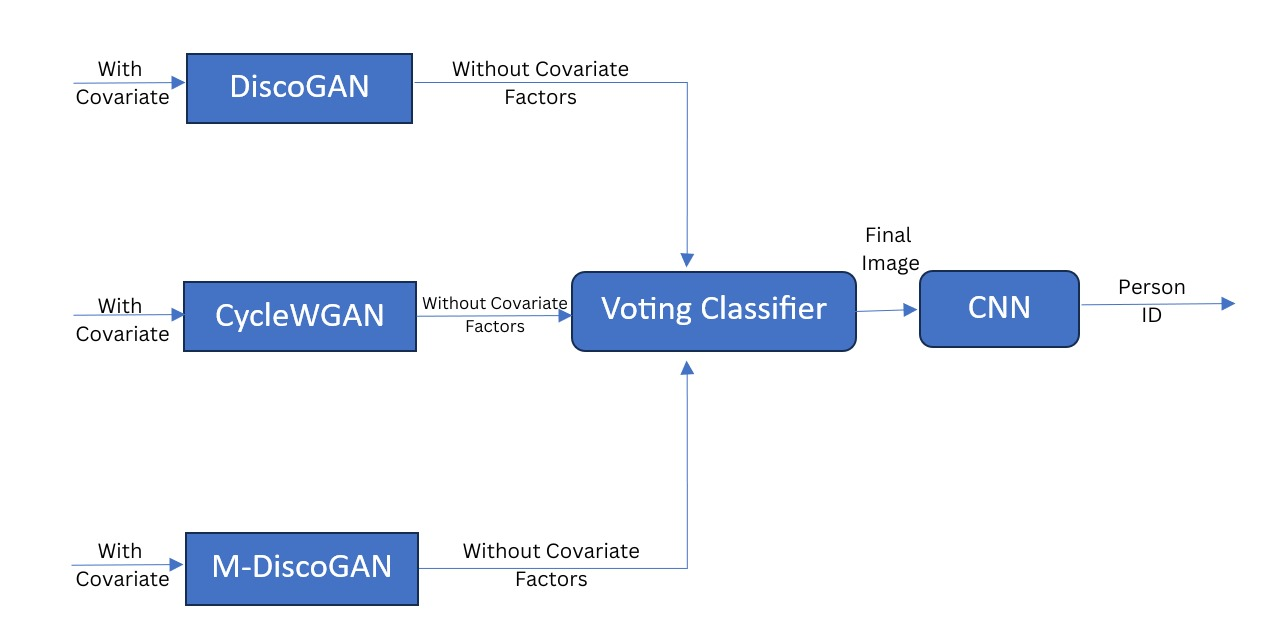
\includegraphics[scale = 0.35]{ppt/img/vc.jpg}
    \caption{Ensemble model of image-to-image translation models combined by a Voting classifier to aggregate the results}
    \label{fig:enter-label}
\end{figure}
\end{frame}

\begin{frame}{CycleWGAN}
\begin{figure}
    \centering
    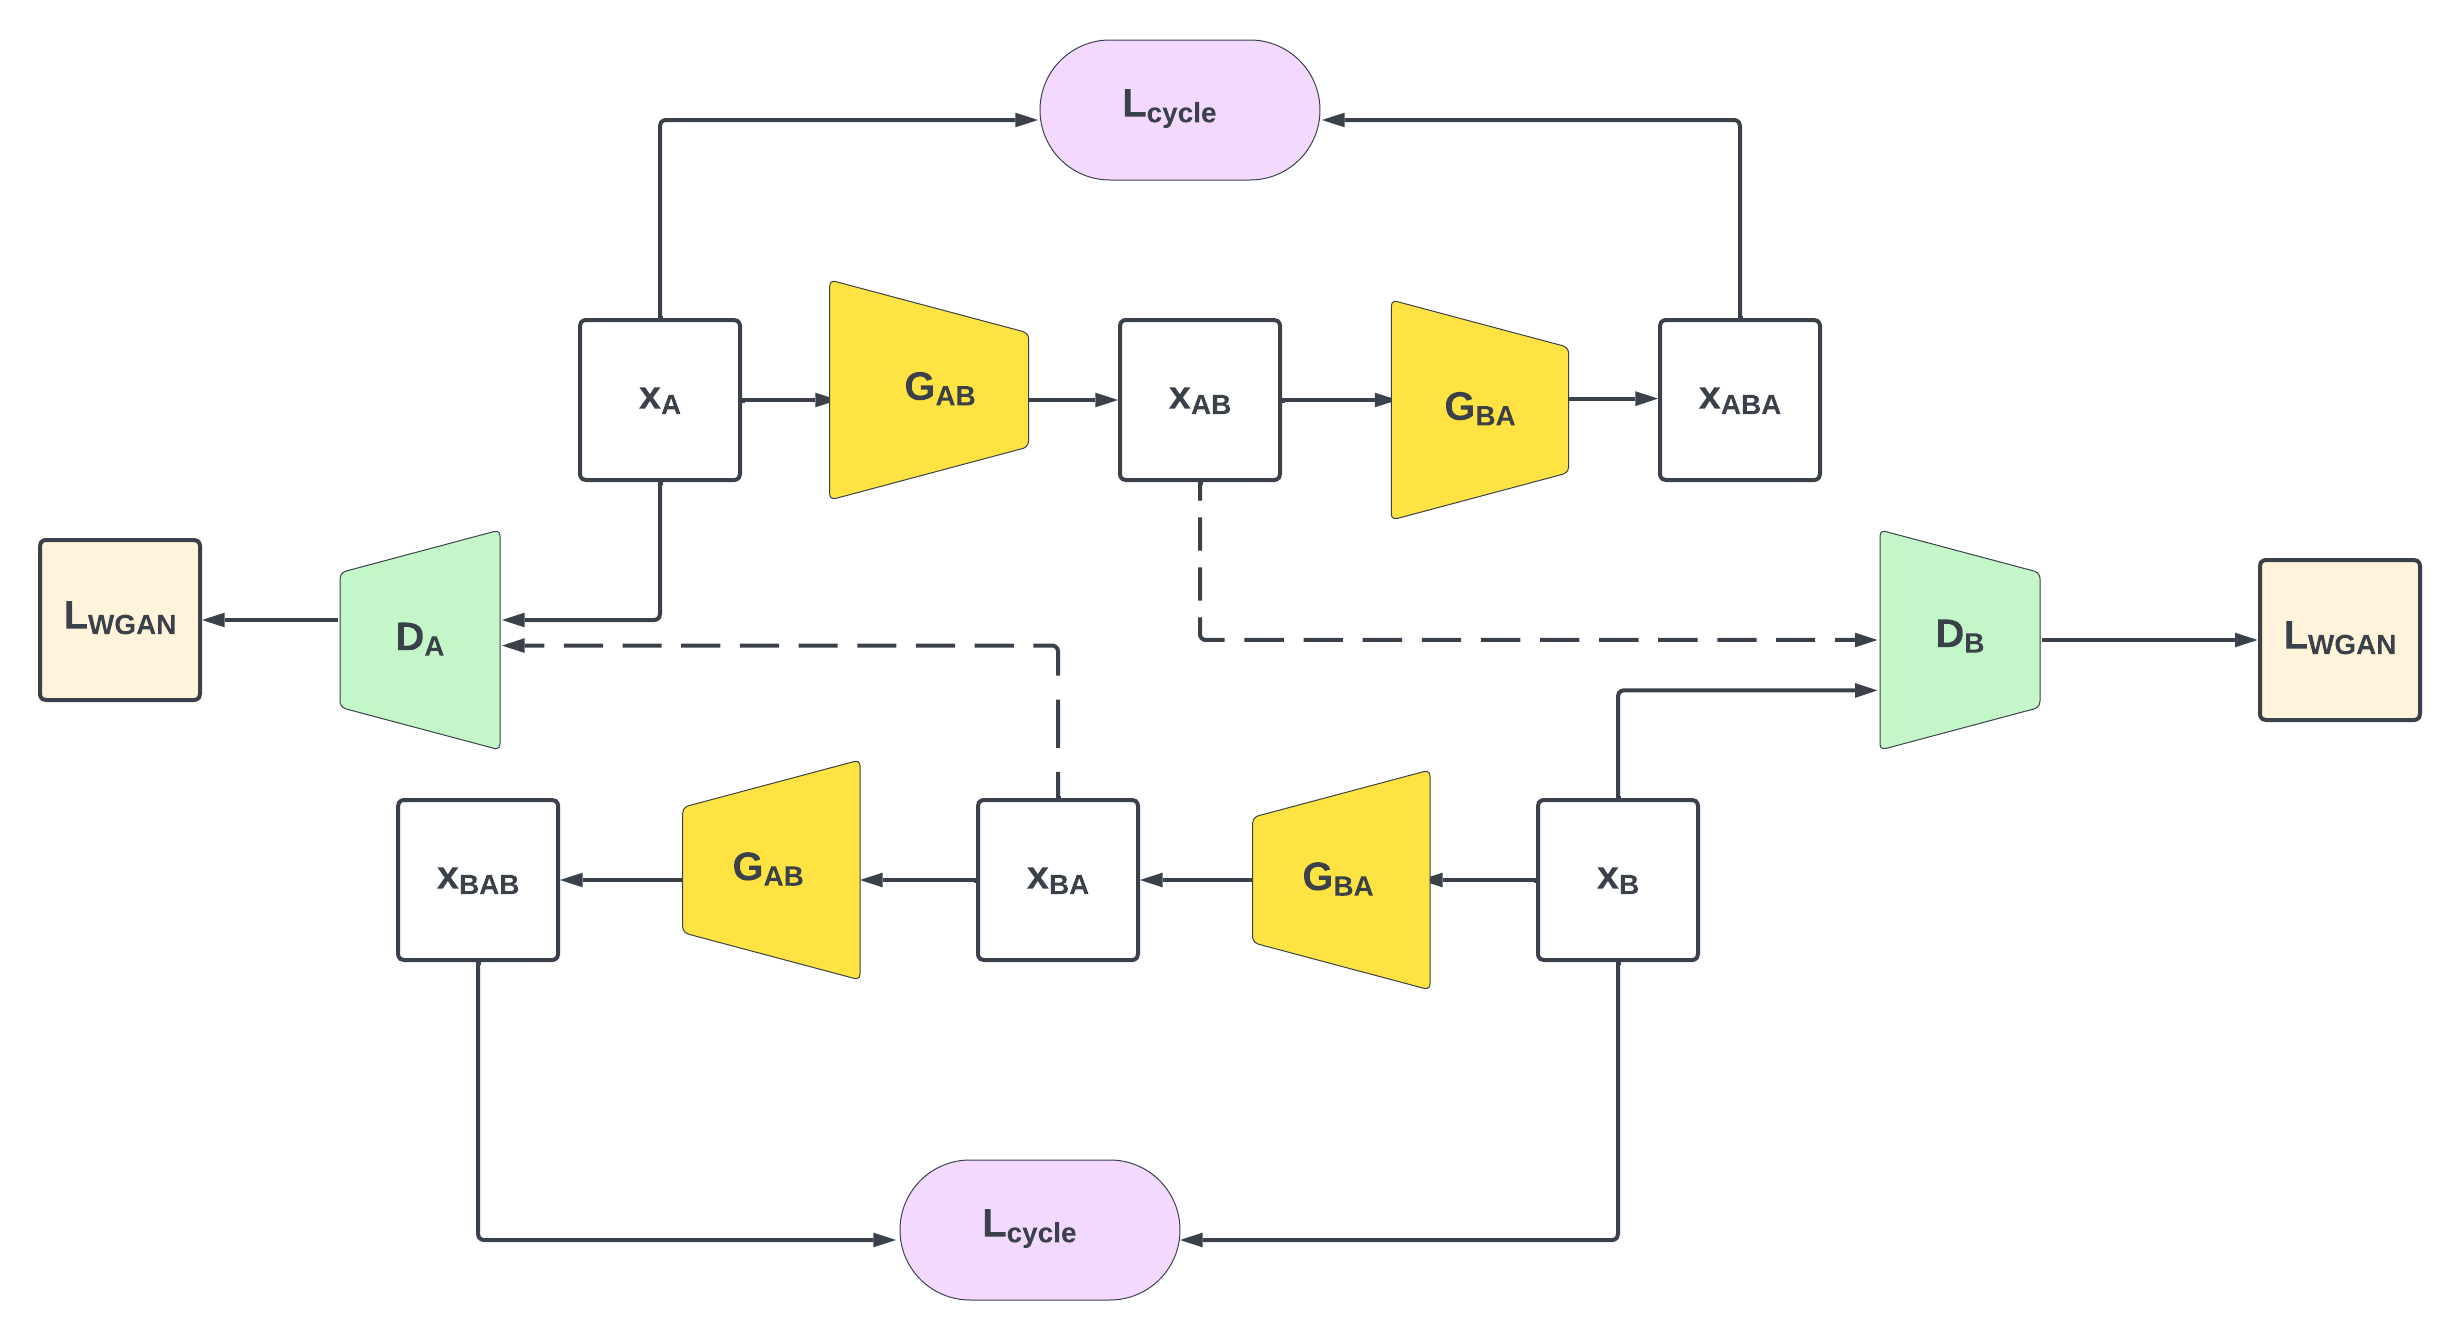
\includegraphics[scale = 0.3]{ppt/img/color-cw.png}
    \caption{Architecture of CycleWGAN}
    \label{fig:enter-label}
\end{figure}
\end{frame}

\begin{frame}{DiscoGAN}
\begin{figure}
    \centering
    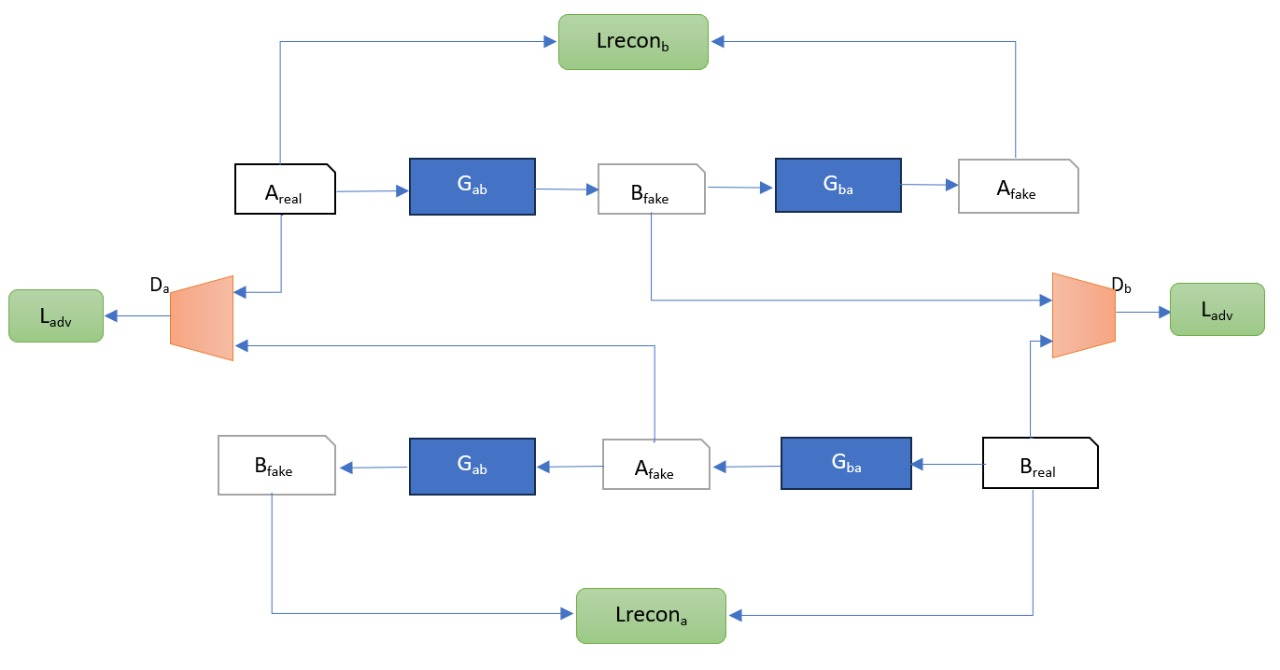
\includegraphics[scale = 0.35]{ppt/img/disco.jpg}
    \caption{Architecture of DiscoGAN}
    \label{fig:enter-label}
\end{figure}
    
\end{frame}



\begin{frame}{M-DiscoGAN}
\begin{figure}
    \centering
    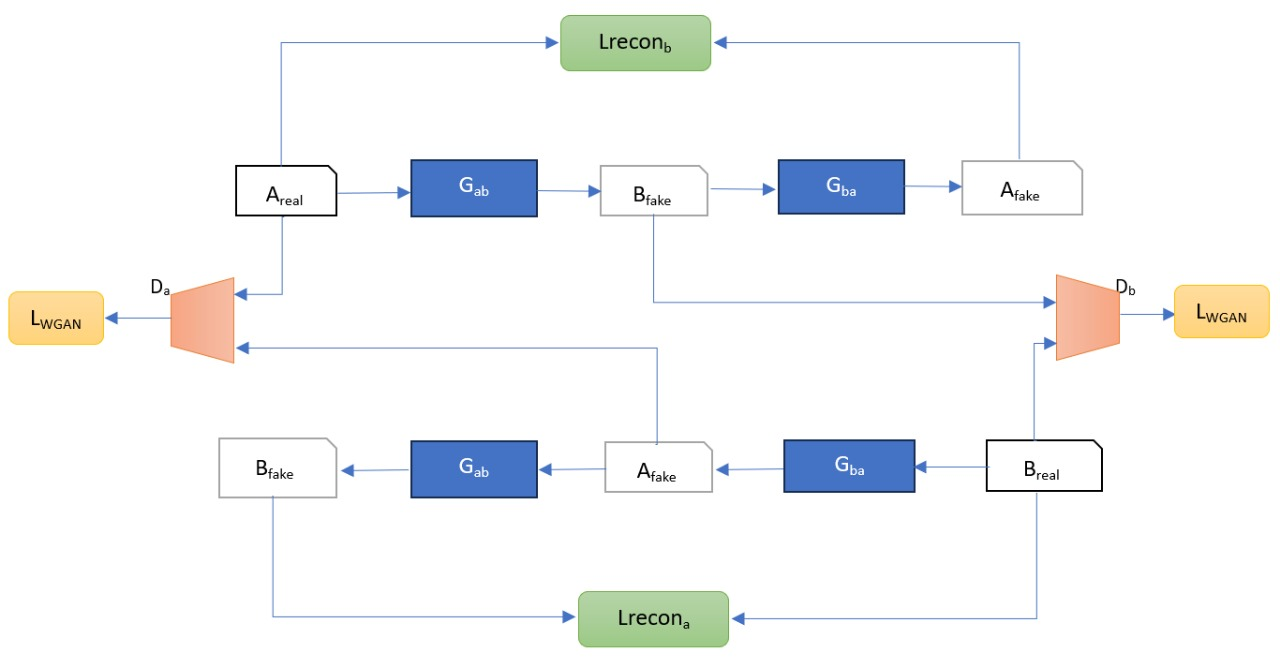
\includegraphics[scale = 0.35]{ppt/img/md.jpg}
    \caption{Architecture of the modified DiscoGAN with Wasserstein loss}
    \label{fig:enter-label}
\end{figure}
\end{frame}

\begin{frame}{Implementation}
\begin{figure}
    \centering
    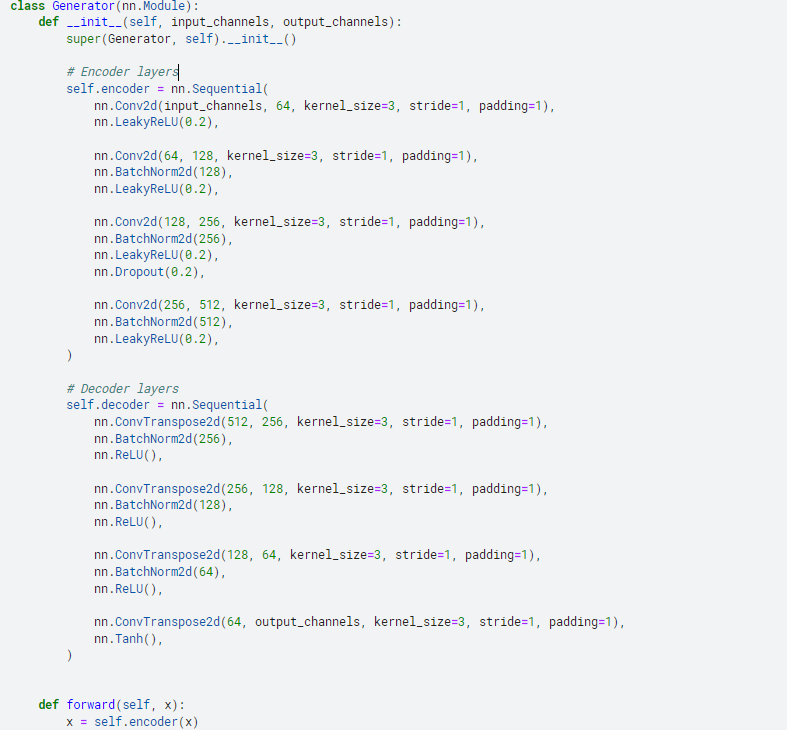
\includegraphics[scale = 0.35]{ppt/Gen.png}
    \caption{Generator architecture}
    \label{fig:enter-label}
\end{figure}
\end{frame}

\begin{frame}{Implementation}
\begin{figure}
    \centering
    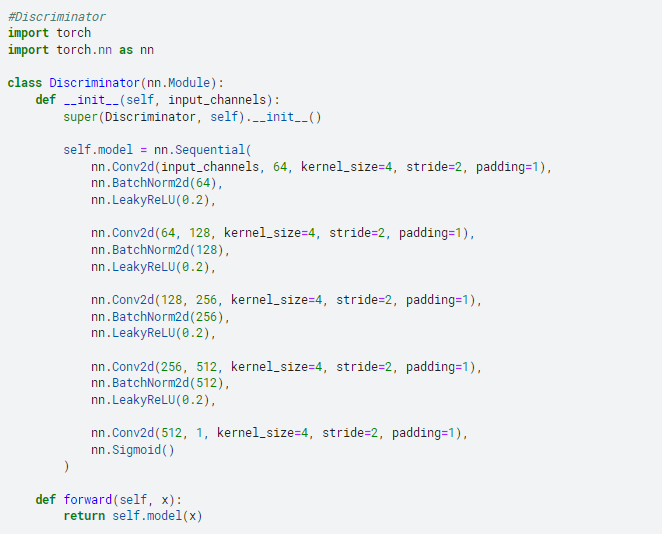
\includegraphics[scale = 0.45]{ppt/Dis.png}
    \caption{Discriminator architecture}
    \label{fig:enter-label}
\end{figure}
\end{frame}

\begin{frame}{Implementation}
\begin{figure}
    \centering
    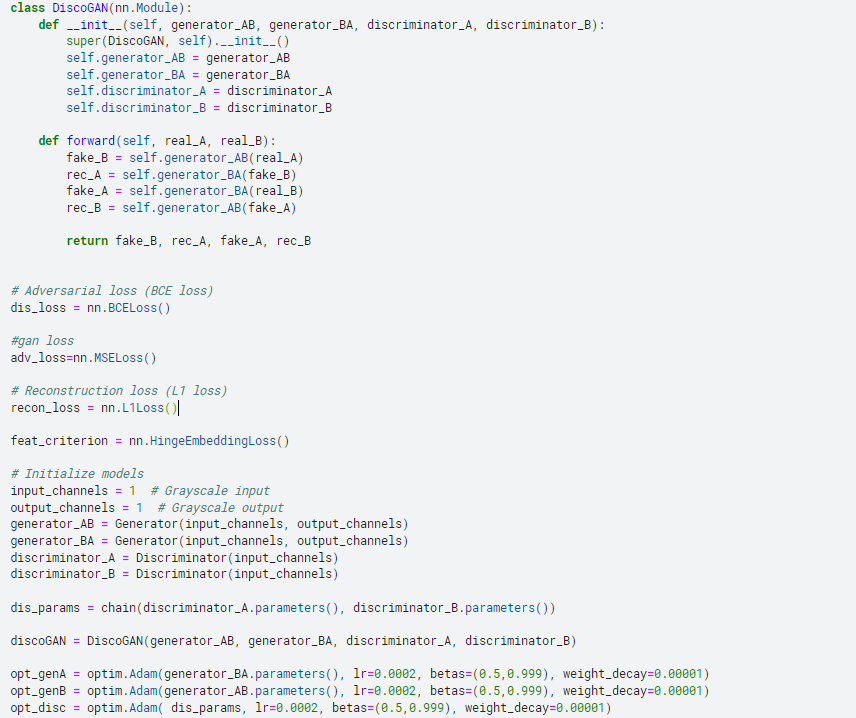
\includegraphics[scale = 0.35]{ppt/DiscoGAN.png}
    \caption{DiscoGAN architecture}
    \label{fig:enter-label}
\end{figure}
\end{frame}

\begin{frame}{Implementation}
\begin{figure}
    \centering
    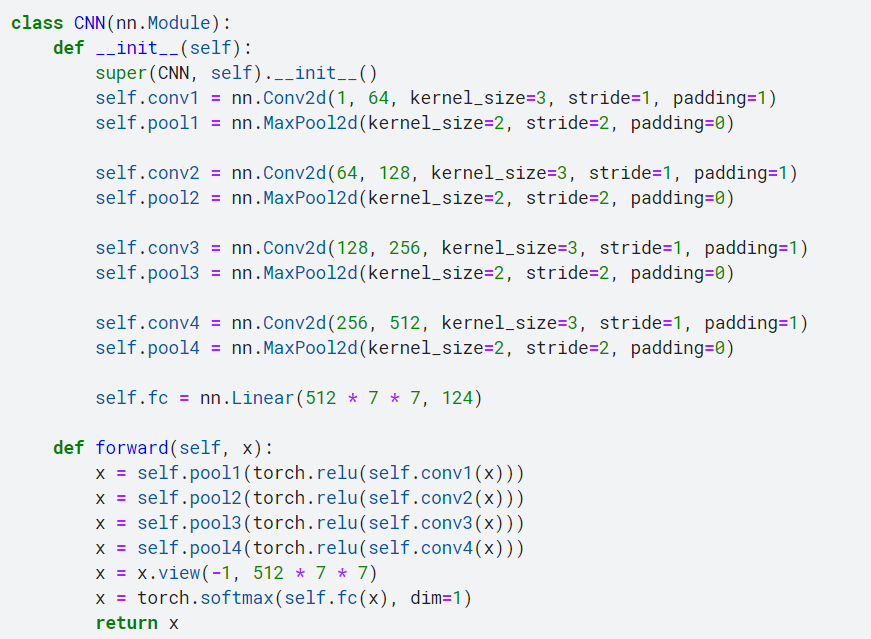
\includegraphics[scale = 0.40]{ppt/CNN.png}
    \caption{CNN architecture}
    \label{fig:enter-label}
\end{figure}
\end{frame}


\begin{frame}{Timeline}
\begin{figure}
    \centering
    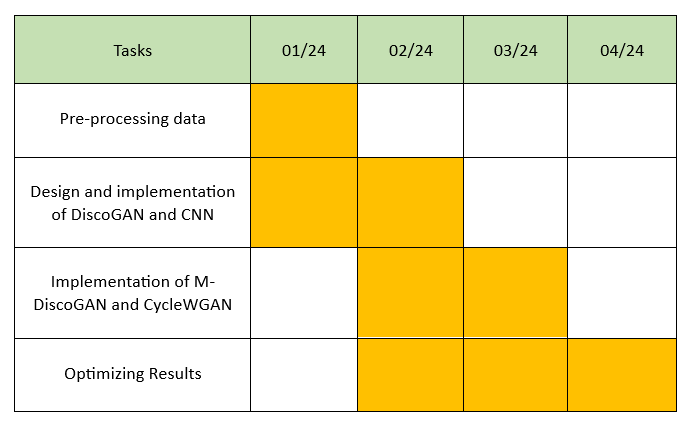
\includegraphics[scale = 0.5]{timeline-chart.png}
    \caption{Project Timeline}
    \label{fig:enter-label}
\end{figure}
\end{frame}



\begin{frame}{References}
\scriptsize
\begin{thebibliography}{99}
  \bibliographystyle{plain}

\bibitem[1] {alsaggaf2021}Alsaggaf, W. A., Mehmood, I., Khairullah, E. F., Alhuraiji, S., Sabir, M. F. S., Alghamdi, A. S., ... Ahmed, A. (2021). A smart surveillance system for uncooperative gait recognition using cycle consistent generative adversarial networks (CCGANs). {\em Computational Intelligence and Neuroscience, 2021.}


\bibitem[2]{kim2017}Kim, T., Cha, M., Kim, H., Lee, J. K., Kim, J. (2017, July). Learning to discover cross-domain relations with generative adversarial networks. {\em In International conference on machine learning (pp. 1857-1865). PMLR.}

\bibitem[3]{arjovsky2017} Arjovsky, M., Chintala, S., Bottou, L. (2017, July). Wasserstein generative adversarial networks. {\em In International conference on machine learning (pp. 214-223). PMLR.}

\bibitem[4] {zou2020} Zou, Q., Wang, Y., Wang, Q., Zhao, Y., & Li, Q. (2020). Deep learning-based gait recognition using smartphones in the wild. {\em IEEE Transactions on Information Forensics and Security, 15, 3197-3212.}


\bibitem [5]{asif2022}Asif, M., Tiwana, M. I., Khan, U. S., Ahmad, M. W., Qureshi, W. S., & Iqbal, J. (2022). Human gait recognition subject to different covariate factors in a multi-view environment. {\em Results in Engineering, 15, 100556.}

\bibitem [6]{vasudevan2023} Vasudevan, P., Mattins, R. F., Srivarshan, S., Narayanan, A., Wadhwani, G., Parvathi, R., & Maheswari, R. (2023). Gait image classification using Deep Learning Models for medical diagnosis.{\em CMC-COMPUTERS MATERIALS & CONTINUA, 74(3), 6039-6063}






\end{thebibliography}
\end{frame}


\begin{frame}{References}
\scriptsize
\begin{thebibliography}{99}
  \bibliographystyle{plain}

\bibitem[7]{khan2023}Khan, M. A., Arshad, H., Khan, W. Z., Alhaisoni, M., Tariq, U., Hussein, H. S., ... & Elashry, A. (2023). HGRBOL2: human gait recognition for biometric application using Bayesian optimization and extreme learning machine.{\em Future Generation Computer Systems, 143, 337-348.}


\bibitem[8] {manssor2021}Manssor, S. A., Sun, S., & Elhassan, M. A. (2021). Real-time human recognition at night via integrated face and gait recognition technologies. Sensors, 21(13), 4323.

\bibitem [9]{huynh2020}Huynh-The, T., Hua, C. H., Tu, N. A., & Kim, D. S. (2020). Learning 3D spatiotemporal gait feature by convolutional network for person identification. {\em Neurocomputing, 397, 192-202.}

\bibitem[10]{wen2022}Wen, J., Shen, Y., & Yang, J. (2022). Multi-view gait recognition based on generative adversarial network. {\em Neural Processing Letters, 54(3), 1855-1877.}

\bibitem[11]{liao2020}Liao, R., Yu, S., An, W., & Huang, Y. (2020). A model-based gait recognition method with body pose and human prior knowledge. {\em Pattern Recognition, 98, 107069.}

\bibitem[12]{zhu2017}Zhu, J. Y., Park, T., Isola, P.,  Efros, A. A. (2017). Unpaired image-to-image translation using cycle-consistent adversarial networks.{\em In Proceedings of the IEEE international conference on computer vision (pp. 2223-2232).}

% \bibitem[13]{hu2021} Hu, W., Li, M.,  Ju, X. (2021). {\em Improved CycleGAN for image-to-image translation.}

\end{thebibliography}
\end{frame}


% \item What is the {\bf Satisfiability Problem} for any Logic?
% \pause
% \item Say Propositional Logic (PL).
% \pause
% \item Given a formula $\alpha$ in PL, 
% \item Does there exists a {\bf valuation} $\nu$ such that $\nu(\alpha)=T$ (i.e., $\nu \models \alpha$)? 
% \end{itemize}
% \end{frame}
% %
% \begin{frame}{Propositional Logic}
% \begin{itemize}
% \item M teaches AI:$~~~~~~M$
% \item S teaches AI:$~~~~~~~S$
% \item M $\&$ S write a book on AI:$~~~~~~~WB$
% %
% \pause
% \item $R=(M\land S)\Implies WB$
% %
% \pause

% \end{itemize}
% \[\{R,\lnot WB,S\}~\mbox{entails}~\lnot M\]
% \pause
% if each of the $\{R,\lnot WB,S\}$ are true then does $\lnot M$ hold?
% \end{frame}

% \begin{frame}{Propositional Logic}
% \begin{itemize}
% \item Does there exist a valuation $\nu$ such that 
% \[\nu \models\{R,\lnot WB,S, M\}\]
% \pause
% \item What is a valuation?
% \pause
% Assignment of {\bf truth values} to $M,S,WB$.
% \pause
% \item Does there exist a valuation $\nu$ such that 
% \[\nu \models R \land \lnot WB\land S\land M\]
% \end{itemize}
% \end{frame}



% \begin{frame}{Propositional Logic}
% \begin{itemize}
% \item Countable set of proposition symbols $P=\{p_1,p_2,p_3,\cdots\}$
% \item Set of propositional connectives $\{\lnot,\lor,\land,\Implies\}$. 
% \end{itemize}
% \pause
% The set of all {\bf well-formed formulas} ({\bf wff}s) of propositional logic are defined inductively as the smallest set satisfying the following conditions:
% \begin{itemize}
% \item Every $p_i \in P$ is a wff, (such wffs are called {\bf atomic formulas})
% \item If $\alpha$ is a wff then $(\lnot \alpha)$ is a wff,
% \item If $\alpha,\beta$ are wffs then so are $(\alpha \lor \beta),(\alpha \land \beta),(\alpha \Implies \beta)$ and
% \item Nothing else is a wff.
% \end{itemize}
% \pause
% Alternatively:
% \[\alpha,\beta \in \Phi::= p_i\in P \mid (\lnot \alpha) \mid (\alpha \lor \beta) \mid (\alpha \land \beta)\mid (\alpha \Implies \beta).\]
% \end{frame}

% \begin{frame}{Propositional Logic:Semantics}
% \begin{itemize}
% \item {\bf valuations} $\nu:P \to \{T,F\}$. 
% \item Every symbol in $P$ gets exactly one of the truth values $\{T,F\}$.
% \end{itemize}
% \pause
% $\nu$ can be extended inductively to the set of all wffs as follows:
% \begin{itemize}
% \item \[ \nu(\lnot\beta)=\left\{ \begin{array}{ll}
%                  T	& \nu(\beta)=F\\
%                  F	& \nu(\beta)=T
                   
%                 \end{array}
%                 	\right. \]
 
% \item \[ \nu(\alpha \lor \beta)=\left\{ \begin{array}{ll}
%                  T	& ~\mbox{when}~ \nu(\alpha)=T ~\mbox{or}~ \nu(\beta)=T\\
%                  F	& otherwise
                   
%                 \end{array}
%                 	\right. \]
 
% \item \[ \nu(\alpha \land \beta)=\left\{ \begin{array}{ll}
%                  T	& ~\mbox{when}~ \nu(\alpha)=T ~\mbox{and}~ \nu(\beta)=T\\
%                  F	& otherwise
                   
%                 \end{array}
%                 	\right. \]

% \item \[ \nu(\alpha \Implies \beta)=\left\{ \begin{array}{ll}
%                  F	& ~\mbox{when}~ \nu(\alpha)=T ~\mbox{and}~ \nu(\beta)=F\\
%                  T	& otherwise
                   
%                 \end{array}
%                 	\right. \]

% \end{itemize}

% \end{frame}

% \begin{frame}{Propositional Satisfiability}
% Given $\alpha$, how do we check the satisfiability of $\alpha$
% \begin{itemize}
% \item Find the set of all propositions occurring in $\alpha$, $P_{\alpha}$,
% \item Generate all possible valuations over $P_{\alpha}$,
% \item There will be $2^{|P_{\alpha}|}$ such valuations,
% \item Check the satisfiability for each such valuation one after another,
% \item If at least one valuation satisfies $\alpha$ (i.e., $\nu(\alpha)=T$, for some $\nu$), \newline report {\bf success}.
% \item If all valuations fail to satisfy $\alpha$ (i.e., $\nu(\alpha)=T$, for all $\nu$), \newline report {\bf failure}.
% \end{itemize}
% \end{frame}
% %
% %
% \begin{frame}{Temporal Logic}
% \begin{itemize}
% \item if M and S teach AI for two consecutive years then eventually they will write the AI book.
% \[\Box \Big(\big((M \land S)\Implies \nxt (M \land S) \big)\Implies \Diamond WB \Big)\]
% \pause
% \item Temporal Modalities
% \begin{itemize}
% \item $\nxt$, $\nxt \alpha$ now if $\alpha$ holds in the immediate future.
% \item $\Box$, $\Box \alpha$ now if $\alpha$ holds {\bf always} in future.
% \item $\Diamond$, $\Diamond \alpha$ now if $\alpha$ holds {\bf sometimes} in future. 
% \end{itemize}
% \end{itemize}
% \end{frame}
% %
% %%----------------------------------------------------------------------------------
% \begin{frame}{LTL Syntax and Semantics}

% \[\psi \in \Psi ::= p \in P \mid  \lnot \psi \mid \psi_1\lor\psi_2 \mid \nxt \psi \mid \Box \psi \mid \Diamond \psi\]
% %\pause

% LTL formulas are interpreted over sequence of valuations 
% \[\nu=\nu_0\nu_1\nu_2\cdots\nu_i\cdots, ~\mbox{where}~ \forall i \in \omega, \nu_i \subset_{fin} P\] 
% \end{frame}

% %----------------------------------------------------------------------------------------------------
% \begin{frame}{Satisfiability Relation}
% \begin{itemize}
% \item $\nu,i\models p$ iff $p \in \nu_i$.
% \item $\nu,i\models \lnot \psi$ iff $\nu,i\not\models \psi$.
% \item $\nu,i\models \psi\lor\psi^{\prime}$ iff $\nu,i\models \psi$ or $\nu,i\models \psi^{\prime}$.
% \item $\nu,i\models \nxt\psi$ iff $\nu,i+1\models \psi$.
% \item $\nu,i\models \Diamond \psi$ iff $\exists j\ge i$, $\nu,j\models \psi$.
% \item $\nu,i\models \Diamond \psi$ iff $\forall j\ge i$, $\nu,j\models \psi$.
% \end{itemize} 
% \[Models(\psi)=\{\nu=\nu_0\nu_1\nu_2\cdots \mid \nu,0\models \psi\}\]
% \end{frame}



% \begin{frame}{LTL Satisfiability}
% Given an LTL formula $\psi$, does there exist a $\nu$ such that \[\nu,0 \models \psi\]
% \begin{itemize}
% \item Construct a B\"uchi Automaton $A_{\psi}$ over $\Sigma=2^{P_{\psi}}$ such that \[Lang(A_{\psi})=Models(\psi)\]
% \item If $Lang(A_{\psi})$ is non-empty then $\psi$ is satisfiable.
% \end{itemize}

% \end{frame}

% \begin{frame}{B\"uchi Automata}
% NFA over infinite words:
% \[B=(Q,\Sigma,\Delta,I,G)\]
% $B$ accepts an infinite word $w \in \Sigma^{\omega}$ if there exists an infinite run $\rho$ of $B$ on $w$ such that some good state $q \in G$ occurs infinitely many times in $\rho$.
% %
% \newline
% \begin{figure}
% \begin{center}
% \begin{tikzpicture}[scale=0.8]
	\node 	(q)		at	(-2,0) 	[circle, thick,minimum size=.75cm]{};

	\node 	(q0)		at	(0,0) 	[circle, thick, draw=blue!50,fill=blue!20,inner sep=0pt,minimum size=.75cm]{$q_0$};


	\node 	(q1)		at	(3,0) 	[circle, thick, draw=blue!50,fill=green!70,inner sep=0pt,minimum size=.75cm]{$q_1$};

	\draw[loop above,very thick] (q0) to 	node[auto]{$a,b$} 		(q0);
	\draw[loop above,very thick] (q1) to 	node[auto]{$a$} 		(q1);
	\draw[->,very thick] (q0) to 	node[auto]{$a$} 		(q1);
	\draw[->,very thick] (q) to 	node[auto]{} 		(q0);

\end{tikzpicture}

% \end{center}
% \end{figure}

% \end{frame}

% \begin{frame}{LTL to B\"uchi Automata}
% Given LTL formula $\psi_0$
% \begin{itemize}
% \item Construct the closure set $cl$ containing
% \begin{itemize}
% \item all subformulas of $\psi_0$
% \item their negations
% \item additional formulas, $\nxt \Diamond \alpha$ if $\Diamond \alpha \in cl$
% \end{itemize}
% \item Define $UR=\{\Diamond \alpha \in cl\}$
% \item Construct the atom set $AT$ as subsets of $cl$ satisfying following criteria:
% \begin{itemize}
% \item for all $\alpha \in cl$, $\alpha \in A$ iff $\lnot \alpha \not \in A$
% \item for all $\alpha \lor \beta \in cl$, $\alpha \lor \beta\in A$ iff $\alpha \in A$ or $\beta \in A$
% \item for all $\Diamond \alpha \in cl$, $\Diamond \alpha \in A$ iff $\alpha \in A$ or $\nxt \Diamond \alpha \in A$
% \end{itemize}

% \end{itemize}

% \end{frame}

% \begin{frame}{LTL to B\"uchi Automata Continued}
% \begin{itemize}
% \item Define $Q=AT \times UR$
% \item Define $I= \{(A,u) \mid \psi_0 \in A,u=\emptyset\}$
% \item Define $G= \{(A,u) \mid u=\emptyset\}$
% \item Define $(A,u)\step{P'}(A',u')$ if the following conditions hold:
% \begin{itemize}
% \item $P'=A \cap P$
% \item for every $\nxt \alpha \in cl$, $\nxt \alpha \in A$ iff $\alpha \in A'$
% \item \[ u'=\left\{ \begin{array}{ll}
%                  \{\Diamond \alpha \in u \mid \alpha \not \in A'\}	& u \not = \emptyset\\
%                  \{\Diamond \alpha \in A' \mid \alpha \not \in A'\}	& u  = \emptyset
                   
%                 \end{array}
%                 	\right. \]

% \end{itemize}
% \end{itemize}
% \end{frame}


\begin{frame}
\begin{center}
{\bf Thank You}
\end{center}
\end{frame}
%
%

\end{document}
